\documentclass[11pt]{report}

\usepackage{caption}
\usepackage{graphicx}
\usepackage{hyperref} 
\usepackage{color}

\marginparwidth 0.5in 
\oddsidemargin 0.25in 
\evensidemargin 0.25in 
\marginparsep 0.25in
\topmargin 0.0in 
\textwidth 6in \textheight 8.5in

\title{sQuire: A Web Based Collaborative Editor\\Homework 7 Individual Work\\Group 3}
\author{Rick Boss (boss2849)}

\begin{document}
\maketitle

\chapter{Personal Work}
\section{Projects Team}
    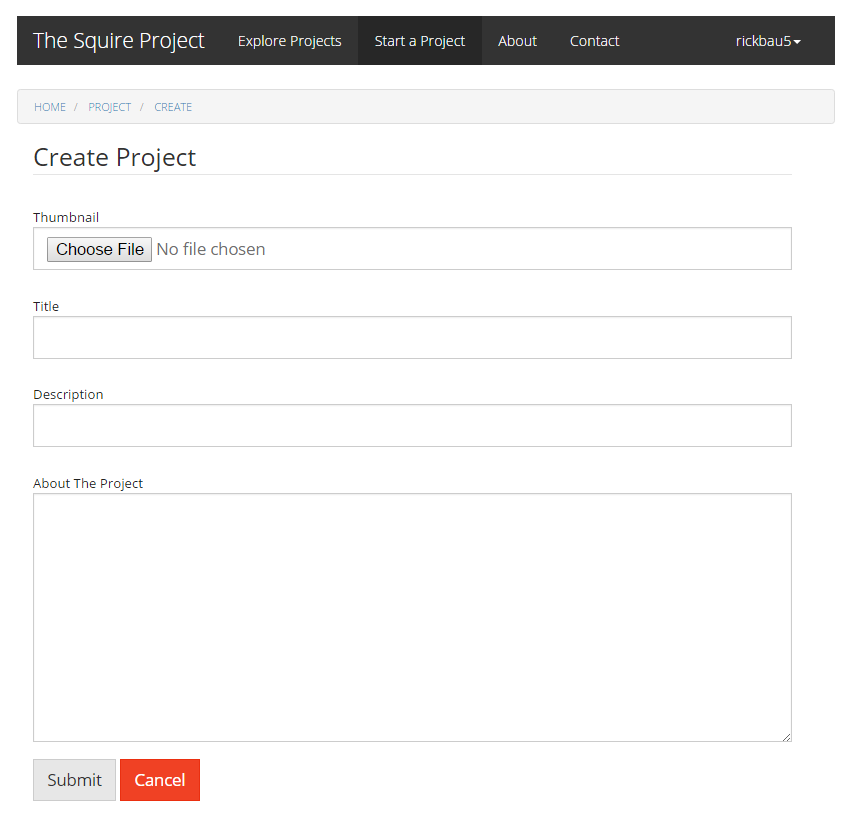
\includegraphics[width=0.9\textwidth]{images/project}
    \\
    \begin{itemize}
        \item Start project: Added image upload, title, description, and body for the user to specify when creating a project. (\color{blue} \href{https://github.com/uidaho/squireproject/pull/47}{\underline{PR 47}}\color{black})
        \item Start project: User must be logged in to start a project. (\color{blue} \href{https://github.com/uidaho/squireproject/pull/47}{\underline{PR 47}}\color{black})
        \item Start project: Implemented title uniqueness requirement. (\color{blue} \href{https://github.com/uidaho/squireproject/pull/47}{\underline{PR 47}}\color{black})
        \item Start project: Implemented length constraints on title, description and body as well as verifying an image is uploaded for thumbnail. (\color{blue} \href{https://github.com/uidaho/squireproject/pull/74}{\underline{PR 74}}\color{black})
        \item Created unit testing for Login, Registration, General permissions, Project creation and viewing. (\color{blue} \href{https://github.com/uidaho/squireproject/pull/75}{\underline{PR 75}}\color{black})
        \item Updated create project, login, register, and reset forms to all use new css theme. (\color{blue} \href{https://github.com/uidaho/squireproject/pull/107}{\underline{PR 107}}\color{black})
        \item Project list: Added pagination, only 16 projects are displayed at a time, the rest overflowing to following pages. (\color{blue} \href{https://github.com/uidaho/squireproject/pull/120}{\underline{PR 120}}\color{black})
        \item Project list: Added sorting, sortable ascending/descending by author, title, and creation/modified dates. (\color{blue} \href{https://github.com/uidaho/squireproject/pull/120}{\underline{PR 120}}\color{black})
    \end{itemize}

\section{Unit Tests}
    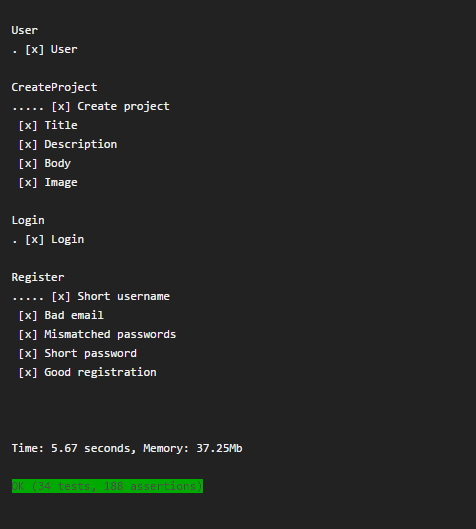
\includegraphics[width=0.9\textwidth]{images/testing} \\
    Majority implemented with \color{blue} \href{https://github.com/uidaho/squireproject/pull/75}{\underline{this pull request.}} \color{black}
    \begin{itemize}
        \item Login: Deny invalid credentials.
        \item Login: Accept valid credentials and redirect.
        \item Project comments: Auth/non-auth users view.
        \item Project creation: Visit as guest.
        \item Project creation: Invalid title.
        \item Project creation: Invalid description.
        \item Project creation: Invalid body.
        \item Project creation: Invalid image.
        \item Project creation: Create valid project.
        \item Project page: Attempt delete project using direct link.
        \item Project page: Attempt delete project as non-owner.
        \item Project page: Delete a valid proejct.
        \item Registration: Invalid username.
        \item Registration: Invald email address.
        \item Registration: Mismatched passwords.
        \item Registration: Invalid password.
        \item Registration: Valid input.
    \end{itemize}


\end{document}
